\documentclass[
	%a4paper, % Use A4 paper size
	letterpaper, % Use US letter paper size
]{IEEEtran}
\usepackage[
backend=biber,
style=alphabetic,
sorting=ynt
]{biblatex}
\addbibresource{reference.bib} %Imports bibliography file

\usepackage{graphicx}
\usepackage{subcaption}
\usepackage{multirow}
\usepackage[utf8]{inputenc}
\usepackage[english]{babel}


\author{Jacob Romero}
\title{Project 1: Supervised learning}

\begin{document}
	%\lsstyle
	\maketitle
	
	\begin{abstract}
		Machine learning has become more pervasive in our everyday life, used for everything from personalized advertising to making financial decisions. In this paper I will compare multiple machine learning algorithms against two data sets, both related to predicting financial information from individuals data. These comparisons will look at how each of the machines learning algorithms performs as more training data is introduced, how each algorithms performs as a function of training time, and lastly a comparison of the algorithms against each other.
	\end{abstract}
	
	\section{Introduction and Problems}
	In this paper I will look at two data sets, and compare these data sets to five different supervised machine learning algorithms. These five algorithms are decision trees, neural networks, boosted decision trees, support vector machines, and k-nearest neighbors. Each algorithm has different properties in the sense of how it models a problem space, its preference bias, expression bias, how fast training and prediction can be done. Finally at the end I will compare these algorithms directly, in order to gain a deeper understanding of how these algorithms are functioning, and some of the trades offs to be made for each of the algorithms.
	
	\subsection{Data set 1}
	The algorithms described previously will be ran and tested against two data sets. The first data set is data from the U.S. census regarding various attributes of an individual. The data set has already been split into two files, a training set, and a testing set. The training set is composed of 32,561 instances, while the testing set has 16,281. Both sets have 14 attributes, these attributes include areas such as age, education level, marital status, occupation, race, sex, etc. From these attributes the final target is whether the individual makes less than or equal to 50 thousand dollars a year, or more than this amount. With a model that can accurately predict an individuals income, or income class in our case would have many uses in other areas, such as targeted marketing, personalized ads, or credit decisions. In addition this problem has some interesting facets to explore, such as what features of this data set contributes to income.
	
	\subsubsection{Feature engineering}
	For this data set the features were pretty clean, as such not much engineering was needed to get to a state where we can input the data into the machine learning algorithms for training. The only pre-processing I did was to convert the discrete columns into one hot encoded features. Allowing our data to be trained on by each of the models. 
	
	\subsection{Data set 2}
	Continuing along the same thing of using machine learning for financial motivations, the second data set again focuses on individuals, but from the other end of the spectrum, in which a customer either defaults on a loan or not. This data set is made up of 24 attributes and is composed of 30,000 instances. Attributes of the data set Include sex, age, marriage status, bill amount for 6 months, payment amount in those 6 months, and the status of the payment during those six months (i.e. paid on time, paid late and by how long, etc.). This again is an interesting problem because the sooner a model can predict possible defaults based, the better chance a lender has of helping the borrower to come to a mutually beneficial arrangement.
	
	\subsubsection{Feature engineering}
	For the second data set, this contained more 'dirty' data and required more pre-processing than was done in data set 1. In addition to the normal one hot encoding of categorical features as was done similarly. This data set had some undefined features in the education level, and marriage features which were denoted with \emph{'?'}, when an unknown bin had already been created. Because the number of instances where these occurred was 14 for the education case, and 54 for in the marriage case for a total of 68 instances with bad data these instances can just be dropped from the data as they only account for 0.2\% of the total data.
	
	Additionally after playing around with training on basic models with default parameters I discovered that, the sex, marriage status, and credit limit balance did not have any affect on the find out come of all of the models. In fact because these features increased the dimensionality of the data it caused decreased performance.
	
	\section{Experiments}
	For this project I was tasked with evaluating and comparing multiple algorithms listed above. Therefore I will train each of the algorithms on each data set also mentioned above, I will evaluate the results of how each algorithm does as a function of training data comparing both the testing, and training data scores. In addition to this, I will compare how two algorithm's performance is affected as hyper-parameters are changed. Specifically I will look at how the max-depth parameter in decision trees, and the number of neighbors used in the K-nearest neighbors classifier. In this paper all performance metrics will be measured in simple accuracy of the models to get the right answer.
	
	\subsection{Methodology}
	For each of the two data set, I will train all five algorithms on the training data set for the first problem, which includes the 32,561 instance. While testing will be done on the second set of 16,281 instances. From there we will compare the training time, performance (accuracy), and hyper parameter tuning performance. While in the second data set because I do not have a second testing set provided, the experiment will still be the same however I will manually split the data set into a training, and testing set using a 80/20 split, where 80\% of the data will be used for training, and 20\% for testing.
	
	\section{Decision Tree Classifier}
		\begin{figure}[h]
			\begin{subfigure}{.5\textwidth}
				\centering
				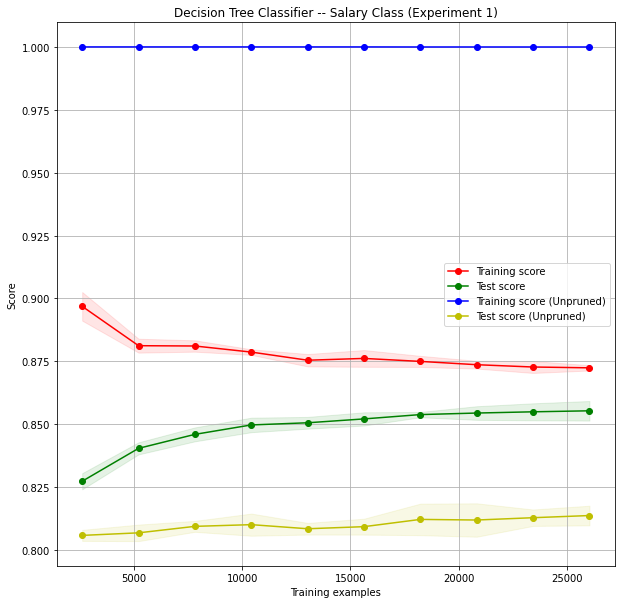
\includegraphics[width=.8\linewidth]{./images/dtExp1.png}
				\caption{Data set 1: Accuracy for training and testing sets on a decision tree model as the number of training data increases.}
				\label{fig:dtexp1}
			\end{subfigure}
			\begin{subfigure}{.5\textwidth}
				\centering
				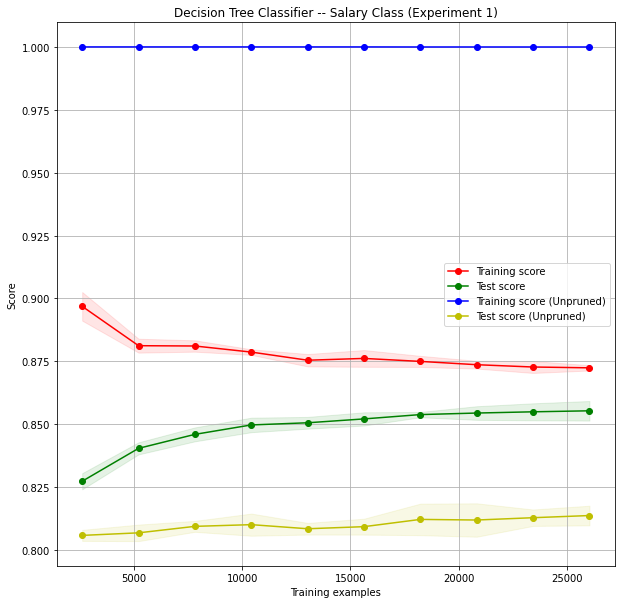
\includegraphics[width=.8\linewidth]{./images/dtExp1.png}
				\caption{Data set 2: Accuracy for training and testing sets on a decision tree model as the number of training data increases.}
				\label{fig:dtexp2}
			\end{subfigure}
		\end{figure}
	
		For the first Algorithm we are looking at decision trees. After training the decision trees, both without pruning and with pruning we get the following:
		\begin{center}
			\begin{table}[h]
				\begin{tabular}{llll}
					& Experiment & Training & Testing \\
					Unpruned & \begin{tabular}[c]{@{}l@{}}Data set 1\\ Data set 2\end{tabular} & \begin{tabular}[c]{@{}l@{}}100.0\%\\ 98.8\%\end{tabular} & \begin{tabular}[c]{@{}l@{}}81.06\%\\ 72.27\%\end{tabular} \\\\
					Pruned & \begin{tabular}[c]{@{}l@{}}Data set 1\\ Data set 2\end{tabular} & \begin{tabular}[c]{@{}l@{}}87.04\%\\ 82.43\%\end{tabular} & \begin{tabular}[c]{@{}l@{}}86.05\%\\ 82.03\%\end{tabular}
				\end{tabular}
			\end{table}
		\end{center}	
		 training accuracy of \emph{unpruned=(100.0\%, 98.88\%)} and \emph{pruned=(87.04\%, 82.43\%)}, (experiment 1, experiment 2). While the testing accuracy numbers show a different story, with \emph{unpruned=(81.06\%, 72.27\%)} and \emph{pruned=(86.05\%, 82.03\%)}. This is interesting but an expected result. It is common knowledge that decision trees can be fast to overfit on data. Because the an unpruned tree will continue to grow when learning on data until it is able to classify all training examples. While when we prune the tree we do see worse training accuracy but improved testing accuracy. Demonstrating the fact that by pruning decision trees we actually get better generalization of the problem. We can see the same results in Figures \ref{fig:dtexp1} and \ref{fig:dtexp2}. In these figures the blue line, representing the accuracy on the training data immediately starts near 100\% accuracy, while we see a 20\% difference in the test score on the same data. While for the pruned tree, as we increase the amount of training data available to our model, we see a slow steady decline in testing score, but a similar inverse increase in the test score, of which has a constantly higher accuracy score than our unpruned tree on the test set.
		
		\subsection{Hyper parameter exploration - Max tree depth}
		\begin{figure}[h]
			\begin{subfigure}{.5\textwidth}
				\centering
				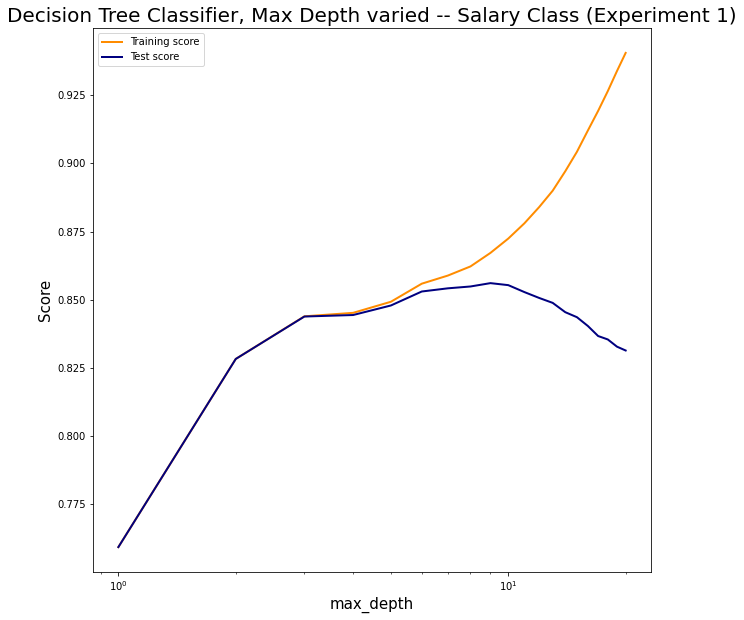
\includegraphics[width=.8\linewidth]{./images/dtMaxDepth1.png}
				\caption{Data set 1: Training and testing accuracy, as the maximum allowed depth of the decision tree is increased.}
				\label{fig:dtDepth1}
			\end{subfigure}
			\begin{subfigure}{.5\textwidth}
				\centering
				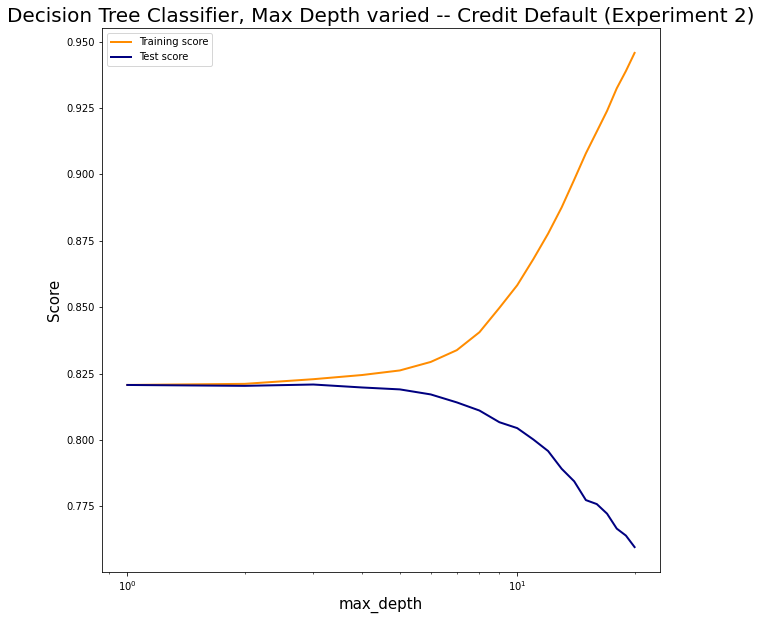
\includegraphics[width=.8\linewidth]{./images/dtMaxDepth2.png}
				\caption{Data set 2: Training and testing accuracy, as the maximum allowed depth of the decision tree is increased.}
				\label{fig:dtDepth2}
			\end{subfigure}
		\end{figure}
		For the second experiment we want to see how effective pruning is at different levels. The previous data showed that a pruned tree generalized better than an unpruned tree, but to what extent does pruning provide increased benefits. In Figures \ref{fig:dtDepth1} and \ref{fig:dtDepth2} these graphs plot the maximum tree depth versus the accuracy score at these various points. For the purpose of this experiment maximum decision tree depth is varied starting from depth 1 to a maximum depth of 20. In both data sets we see that as the tree is allowed to grow longer we see an increased testing score. But eventually a drop in the testing score. However, the interesting thing to note is that in the first data set we see an increase in accuracy gains for both the training and testing scores as we increase the max depth for the tree up to a depth fo 10. After which the training score continues to increase as the test score decreases. This is expected as we since when we increase the depth of the tree we create more opportunities for our tree to overfit.
	
	\section{K Nearest Neighbors Classifier}
		\begin{figure}[h]
			\begin{subfigure}{.5\textwidth}
				\centering
				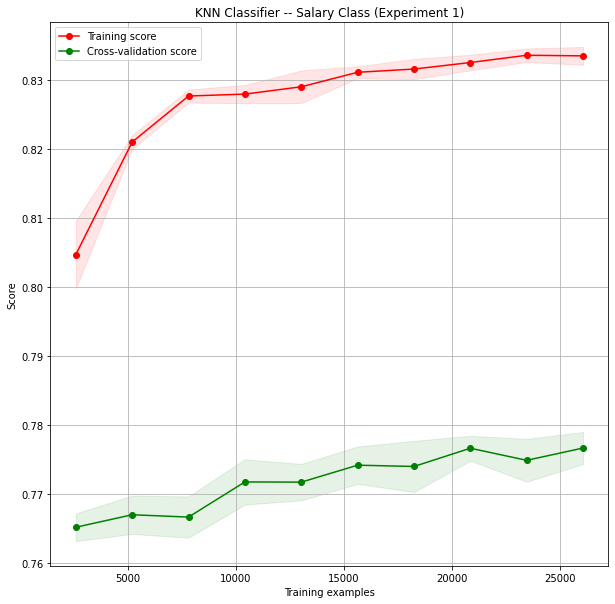
\includegraphics[width=.8\linewidth]{./images/knnExp1.png}
				\caption{Data set 1: KNN model's accuracy (Against train and test sets), as training set size increases.}
				\label{fig:knnExp1}
			\end{subfigure}
			\begin{subfigure}{.5\textwidth}
				\centering
				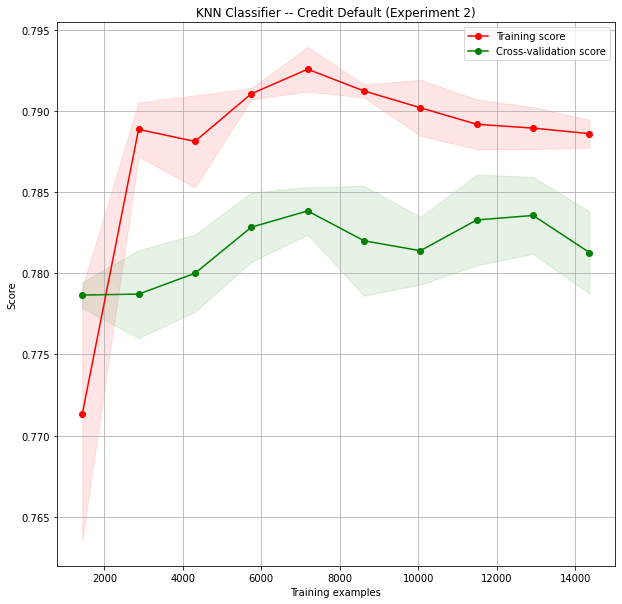
\includegraphics[width=.8\linewidth]{./images/knnExp2.png}
				\caption{Data set 2: KNN model's accuracy (Against train and test sets), as training set size increases.}
				\label{fig:knnExp2}
			\end{subfigure}
		\end{figure}
	
		Unlike the other algorithms in this paper K nearest neighbors is an instance based algorithm, so rather than trying to eagerly learn from the data we pass into the algorithm, instead the data is stored in memory. When a prediction is attempted to be made the algorithm will then query its memory for the \emph{K} closest neighbors and use the values from those neighbors to make a prediction. After training the model on both data sets, the results are the following:
		\begin{center}
			\begin{table}[h]
				\begin{tabular}{lll}
					Experiment & Training & Testing \\
					Data set 1 & 99.99\% & 77.11\% \\
					Data set 2 & 78.85\% & 77.57\%
				\end{tabular}
			\end{table}
		\end{center}
		The benefit of this approach of using instance based learning is as we add more data points, the better our predictions should typically do under the assumption that there is correlations between our features to the target outcome. We can this shown in the Figures \ref{fig:knnExp1}/\ref{fig:knnExp2}. In both of these graphs we see how by adding more training data to the model drives up performance. However we see more of an increase in gains of adding training data in our first data set over the second data set. This can be attributed possibly to the fact that as mentioned points, and features may be more strongly correlated in the salary data set, over the credit default data set. However there are drawbacks to the lazy learning method of KNN, particularly in the time it takes for the model to make a prediction, and memory requirements for large data sets. We will explore the aspect of long prediction times later on in this paper. However the memory requirements as mentioned includes storing all data in memory for use later when making a prediction. This means that if we have a data set consisting of hundreds of gigabytes or even terabytes, this means the computer must have enough ram to store the data, or it must continually page in and out data from memory.
	
		\subsection{Hyper parameter exploration - K neighbors parameter}
			\begin{figure}[h]
				\begin{subfigure}{.5\textwidth}
					\centering
					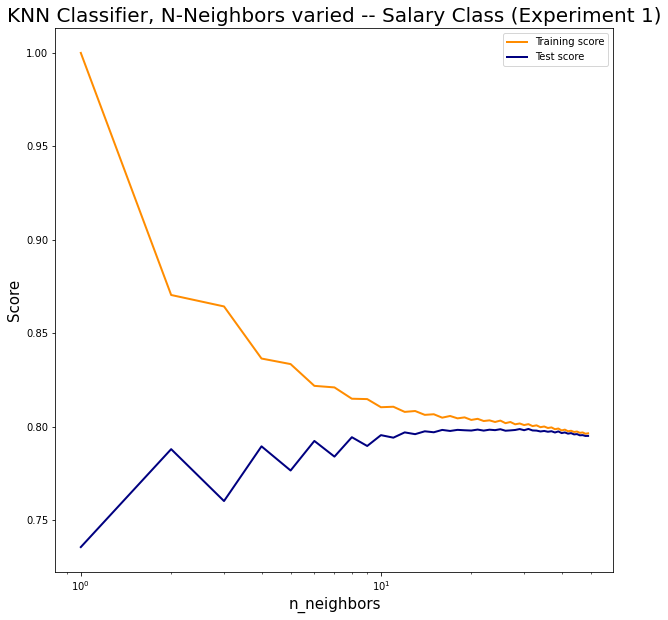
\includegraphics[width=.8\linewidth]{./images/knnNeghbors1.png}
					\caption{Data set 1: K neighbors hyper parameter exploration and the affect on accuracy}
					\label{fig:knnNeighbors1}
				\end{subfigure}
				\begin{subfigure}{.5\textwidth}
					\centering
					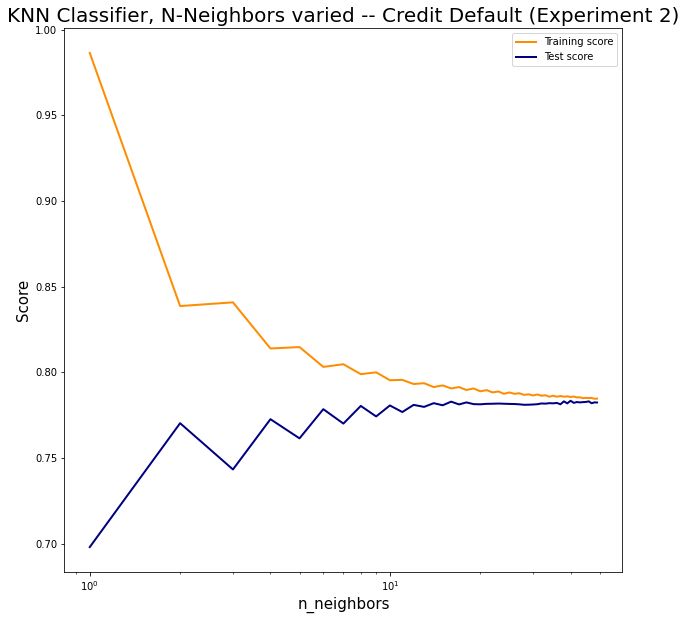
\includegraphics[width=.8\linewidth]{./images/knnNeghbors2.png}
					\caption{Data set 2: K neighbors hyper parameter exploration and the affect on accuracy}
					\label{fig:knnNeighbors2}
				\end{subfigure}
			\end{figure}
			The \emph{K} in the K-nearest neighbors name refers to the number of nearest datapoints to look at when making a prediction. This can change how our model decides the output of a prediction by including more factors in the output selection process, or voting process. Such as using five of the nearest neighbors may be close to the target. However if we look at 10 neighbors where 5 are close in approximation to the target, but the other 5 are opposite to our target output we could result in a tie, in which we need to break it, that may lead to choosing the wrong label. We explore this by taking our KNN algorithm and running it over the data using various values of \emph{K}. For our testing purposes we adjust the value of \emph{K} from 1, to 50 neighbors. The results of which are shown in Figures \ref{fig:knnNeighbors1} and \ref{fig:knnNeighbors2}. We see some interesting outcomes from doing this experiment. For the first data set, we at first see a moderate increase in gains for the testing, and sharp decreases in values from our training set. Because increasing the size of the voting pool reduces overfitting. Because KNN with a value of \emph{k=1} the algorithm is nothing more than a lookup table which returns the exact instance we have put in memory from our training data. However increasing values of \emph{k} increases the generalization by allowing more of the close neighbors to contribute to the output. But this comes at the cost that our exact values are no longer solely returned by our algorithm.
	
	\subsection{Neural Network Classifier}
		\begin{figure}[h]
			\begin{subfigure}{.5\textwidth}
				\centering
				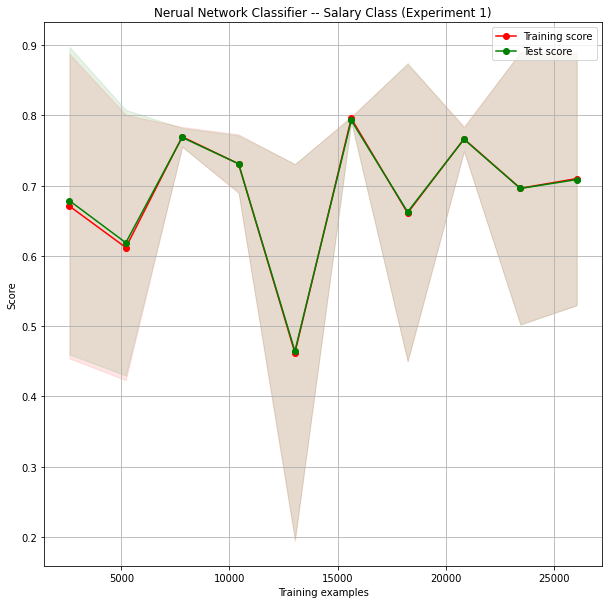
\includegraphics[width=.8\linewidth]{./images/nnExp1.png}
				\caption{Data set 1: Neural network accuracy score as a function of training set size.}
				\label{fig:nnExp1}
			\end{subfigure}
			\begin{subfigure}{.5\textwidth}
				\centering
				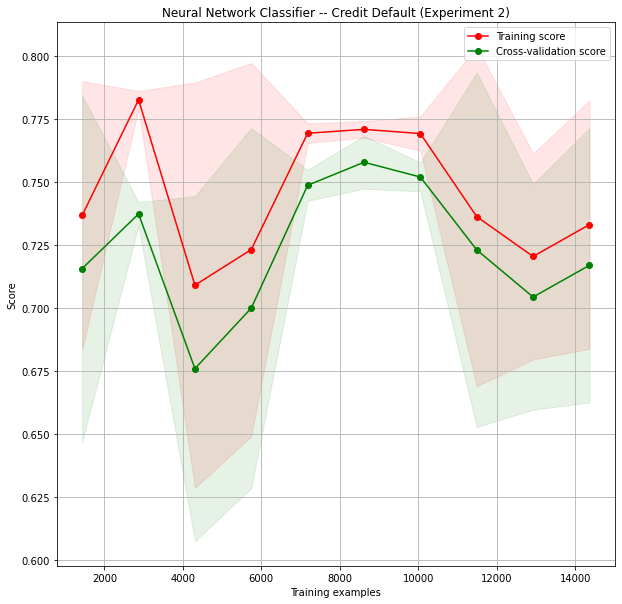
\includegraphics[width=.8\linewidth]{./images/nnExp2.png}
				\caption{Data set 2: Neural network accuracy score as a function of training set size.}
				\label{fig:nnExp2}
			\end{subfigure}
		\end{figure}
		Neural networks have become the standard ML algorithm in practice today due to their flexibility and expressiveness for problem spaces. Neural networks are capable of expressing simple equations, all the way to extremely complex equations by altering the structure of the network. A neural network has two parameters to its structure, the number of hidden layers in the network, and the number of nodes in each layer also called the layer's size. Because of the complexity of the equations that a neural network can express they are typically black box models. In which understanding why a certain output is received is not usually possible. There is also the fact that neural network training requires finding local minima but does not guarantee finding the global optimum of a function. We can see this in effect on the figures from this experiment (Figures \ref{fig:nnExp1}/\ref{fig:nnExp2}). As more training data is fed into the model we see a slight but jagged upward trend on the accuracy score of the model, this occurs in both the data sets. An interesting note however is that the training and cross validation are very close in value from a low amount of training data. This could be due to the fact that the network does not need a large amount of training data to converge. While the jagged peaks and troughs could be cause by the randomness in the learning algorithm. For the final result we can get the following data.
		
		\begin{center}
			\begin{table}[h]
				\begin{tabular}{lll}
					Experiment & Training & Testing \\
					Data set 1 & 81.35\% & 81.47\% \\
					Data set 2 & 76.02\% & 74.51\%
				\end{tabular}
			\end{table}
		\end{center}
	
	\subsection{Boosted Decision Tree Classifier}
		\begin{figure}[h]
			\begin{subfigure}{.5\textwidth}
				\centering
				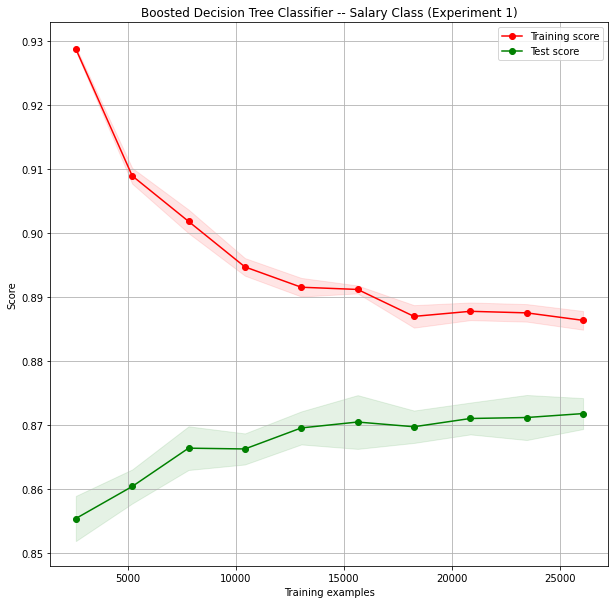
\includegraphics[width=.8\linewidth]{./images/bdtExp1.png}
				\caption{Data set 1: Accuracy of Boosted Decision trees, as a function of training set size. This graph shows the power of boosting, even with a large data set the test set score is still on an upward trend}
				\label{fig:bdtExp1}
			\end{subfigure}
			\begin{subfigure}{.5\textwidth}
				\centering
				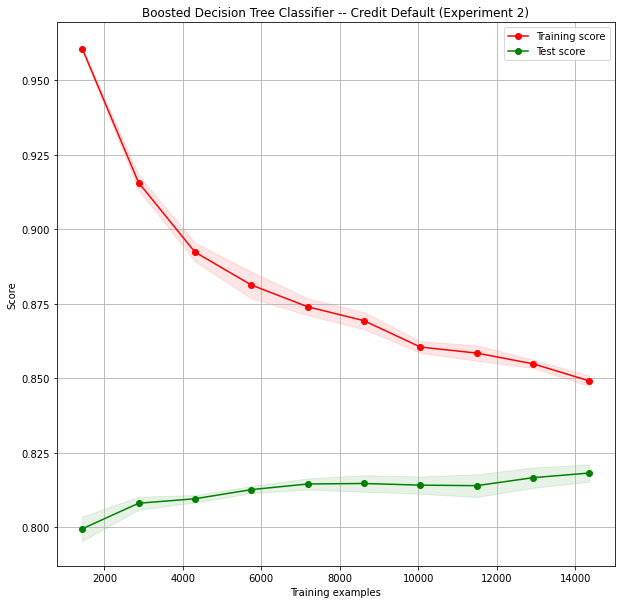
\includegraphics[width=.8\linewidth]{./images/bdtExp2.png}
				\caption{Data set 2: Accuracy of Boosted Decision trees, as a function of training set size. Similar pattern as data set 1, showing an upward trend even in a large data set.}
				\label{fig:bdtExp2}
			\end{subfigure}
		\end{figure}
		Boosted decision trees is the most interesting of the algorithms as this one has the highest accuracy of all the algorithms. Possibly due to the fact that boosting allows the learning to constantly increase its learning capability. As we have seen in the lectures ensemble learning, such as in boosted decision trees, requires that new learners be at least better than chance at predicting the data. This means that as more data is added to the learner it will never overfit. Because both of my data sets are relatively larger, the boosting algorithm is able to take full advantage of this and learn as much as possible. As a result the final outcome of running the algorithm over my data sets is:
		\begin{center}
			\begin{table}[h]
				\begin{tabular}{lll}
					Experiment & Training & Testing \\
					Data set 1 & 88.42\% & 87.52\% \\
					Data set 2 & 84.38\% & 81.80\%
				\end{tabular}
			\end{table}
		\end{center}
		We can see the effects of boosting in the graphs for these algorithms at Figures \ref{fig:bdtExp1}/\ref{fig:bdtExp2}. In which the graph is monotonically increasing even at the last data point. However we can note that the amount of increase from add more data to the learning is diminished for the more data we add.
	\subsection{Support Vector Classifier}
		\begin{figure}[h]
			\begin{subfigure}{.5\textwidth}
				\centering
				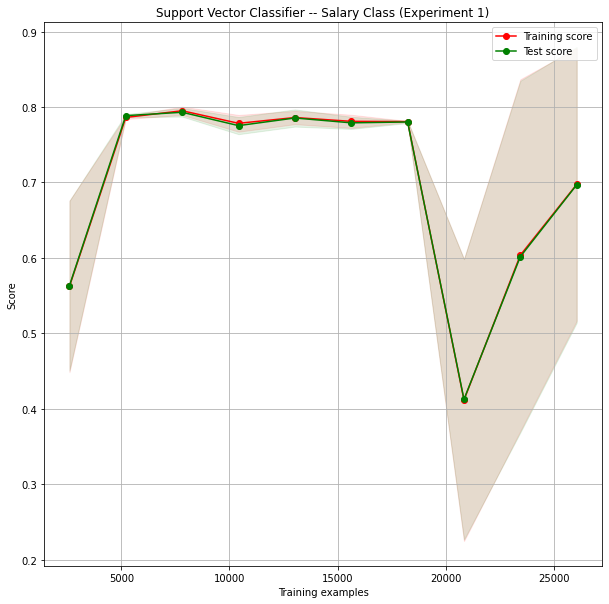
\includegraphics[width=.8\linewidth]{./images/svcExp1.png}
				\caption{Data set 1: SVC accuracy score, as training data increases. Interestingly enough there doesn't seem to be any gain from increasing the training data size.}
				\label{fig:svcExp1}
			\end{subfigure}
			\begin{subfigure}{.5\textwidth}
				\centering
				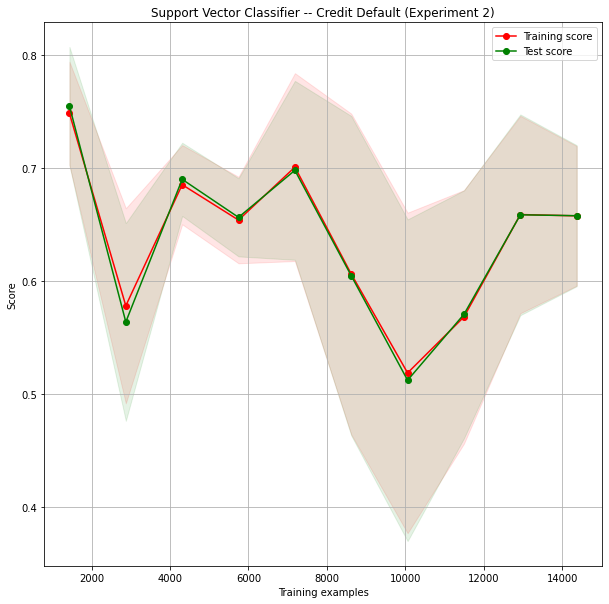
\includegraphics[width=.8\linewidth]{./images/svcExp2.png}
				\caption{Data set 2: SVC accuracy score, as training data increases. Reinforces the idea that for these data sets Linear SVC may not be sophisticated enough to predict these data sets.}
				\label{fig:svcExp2}
			\end{subfigure}
		\end{figure}
		Support vector machines from my experience have usually been fairly powerful, but from the scikit-learn\cite{scikit-learn} documentation do not scale well with large data set, both of the ones we are using fit this description, " The fit time scales at least quadratically with the number of samples and may be impractical beyond tens of thousands of samples". Because of this I was limited in the scope of the testing I was able to perform on these. For this experiment we see the same general trend of adding more training data results in a general overall higher score. But there are two interesting points here. First is the data set 1, in Figure \ref{fig:svcExp1}, shows a strong increase in the accuracy score gained as more data is added, this is interesting as the graph appears to have a trend of flattening but not as much as is expected. This could be due to the time constraints of running the algorithm with such a large data set and the training times being long, I manually capped the number of training iterations at 1000. As such when the size of the data is larger, there is a greater chance the algorithm can pick out more information. The final results of training the support vector machine is,
		\begin{center}
			\begin{table}[h]
				\begin{tabular}{lll}
					Experiment & Training & Testing \\
					Data set 1 & 78.20\% & 78.52\% \\
					Data set 2 & 67.10\% & 66.39\%
				\end{tabular}
			\end{table}
		\end{center}
		As mentioned previously because of the large amount of data in the data sets I choose running exhaustive tests on support vector classifiers was limited, demonstrating the draw backs of this algorithm. Additionally training was limited to a linear support vector classifier, and in light of the not so great scores (compared to other algorithms), leads me to believe that this problem is not easily linearly separated by the data, especially in data set 2.
	
	\subsection{Results, Analysis, \& Comparison}
	Finally after going through all the algorithms individually, we have seen the powers, some of the drawbacks, and even some weird quirks with each of the algorithms on their own. But to get full insight into each algorithm we need to compare them to each other. We will also need to look other metrics instead of how accurately the models predicted the output of training data. Although that is still an important metric, as such let start by comparing the the models to each other. In Figure \ref{fig:allAgsTrainAcc} we can see how each model does when testing on their training data. This gives us insight into how well the these models may generalize. Specifically looking at Unpruned decision trees, and KNN, we see perfect scores of about 1.0 or 100\% prediction accuracy (data rounted to 4 decimal points). This was detailed above but to recap, decision trees that are unpruned will learn all of the features in order to correctly classify their training data, leading to overfitting. While in the KNN case, because of the low number of neighbors and the feature of the algorithm to recall exact data points from memory this gives extremely high training scores.
	
	But looking at the accuracy scores on the testing data provides a better reality of how each of these algorithms generalize. In Figure \ref{fig:allAgsTestAcc} we can see the comparison here. The story is vastly different for the two algorithms above, unpruned decision trees is now one of the wort performing algorithms near on par with support vector classifier. However KNN does still generalize pretty well in comparison to other algorithms, even though it does well on test data due to the fact that it can recall exact training data as mentioned. However the standout is boosted decision trees, as we have seen previously it is able to make use of the large data sets to generalize particularly well in data set 1.
	\begin{figure}[h]
		\begin{subfigure}{.5\textwidth}
			\centering
			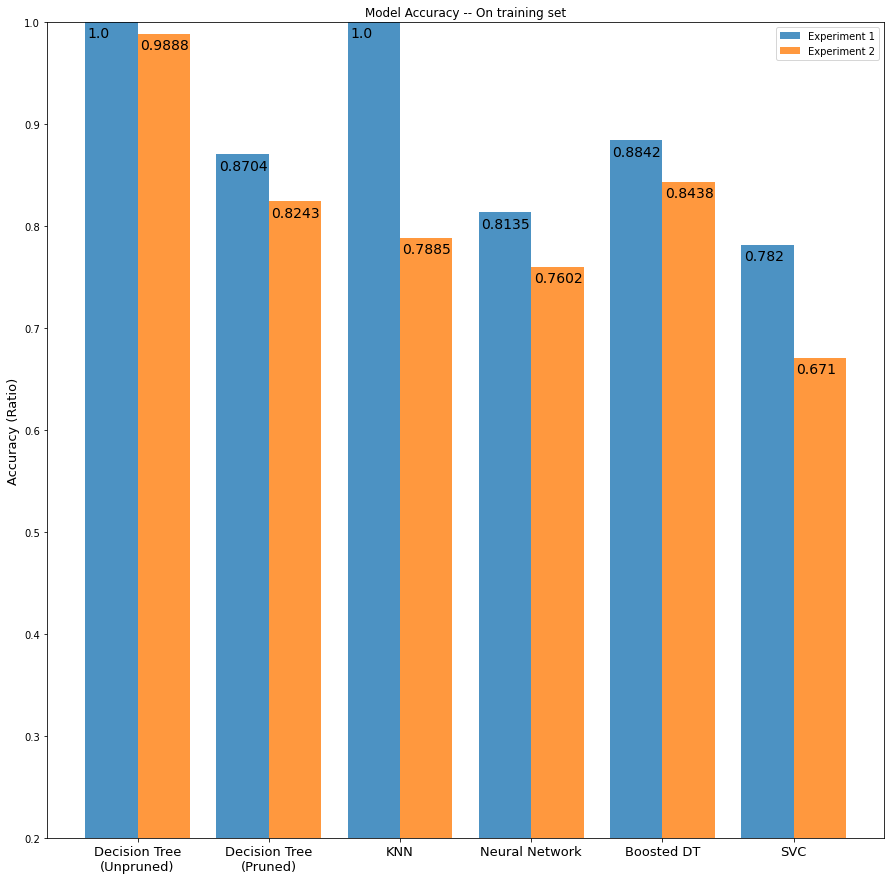
\includegraphics[width=.8\linewidth]{./images/allModelsTrainingAcc.png}
			\caption{All supervised learning algorithms training set accuracy scores.}
			\label{fig:allAgsTrainAcc}
		\end{subfigure}
		\begin{subfigure}{.5\textwidth}
			\centering
			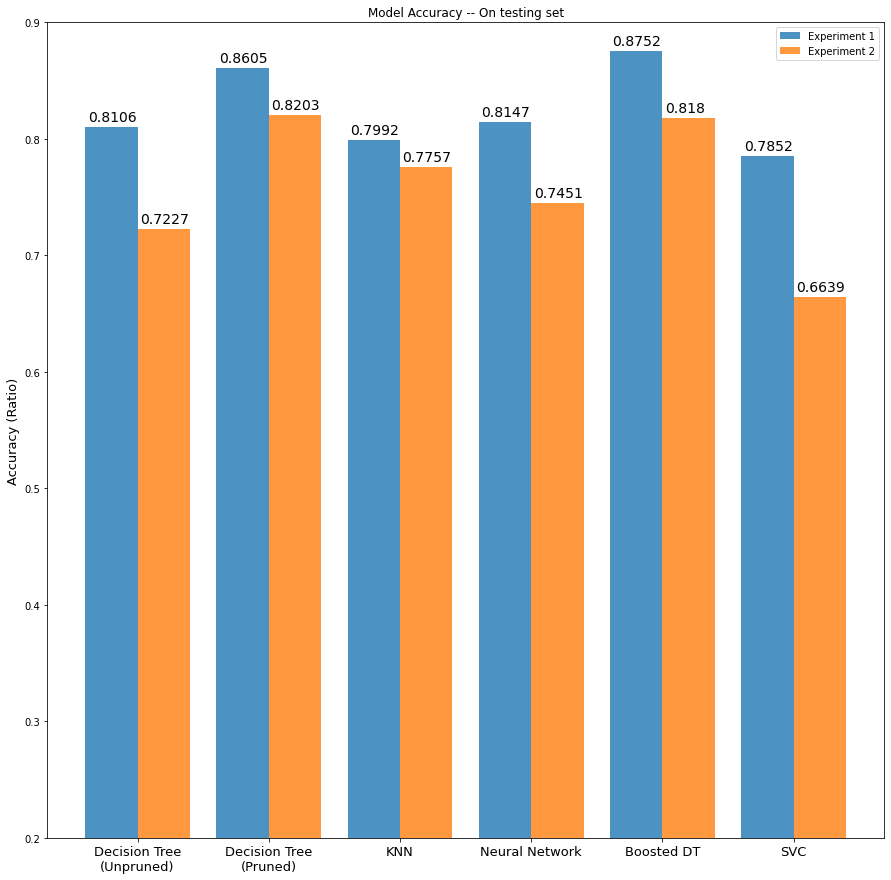
\includegraphics[width=.8\linewidth]{./images/allModelsTestAcc.png}
			\caption{All supervised learning algorithms testing set accuracy scores.}
			\label{fig:allAgsTestAcc}
		\end{subfigure}
	\end{figure}

	As we have been looking solely at accuracy across the models, I will end the paper by looking at two different metrics. First in Figure \ref{fig:allAgsTrainTime} we have the time taken (in seconds) to train all the models on each of the full data sets. From here we can highlight some of the key pros not revealed in the training data. In particular we can see the training time for KNN is non-existent, due to the fact that 'training' a KNN model simply involves a storage call for the data points. Where as we can see how Neural networks can take a long time, this is especially true as you start to increase the complexity of the network. Finally the worst offender the support vector classifier take the mose time at 9.47 seconds for the first data set, and 14.68 seconds for the second data set. This is particularly attributed to the fact that the data was not linearly separable, and as such the algorithm could not converge taking the full amount of iterations before forcefully exiting the training.
	
	However looking at training time is not the full picture still, to get there we also need to consider the time it takes to make a prediction. In Figure \ref{fig:allAgsTestTime}, we have exactly that data. In this is where we can see the real drawback of using a KNN model for predictions. In this case the time taken to predict the full data set was, 4.3274 seconds for data set 1, and 10.116 seconds for data set 2. This means that if an application is prediction heavy and sensitive to long latency KNN will almost always not deliver on time. This fact is compounded more so as you add more data to the model. While on the other side of things we can see how simpler models like decision trees and linear support vector classifiers can actually provide much needed boost to prediction speeds. Taking anywhere around 0.002-0.003 seconds to predict the large testing sets used in the experiments.
	\begin{figure}[h]
		\begin{subfigure}{.5\textwidth}
			\centering
			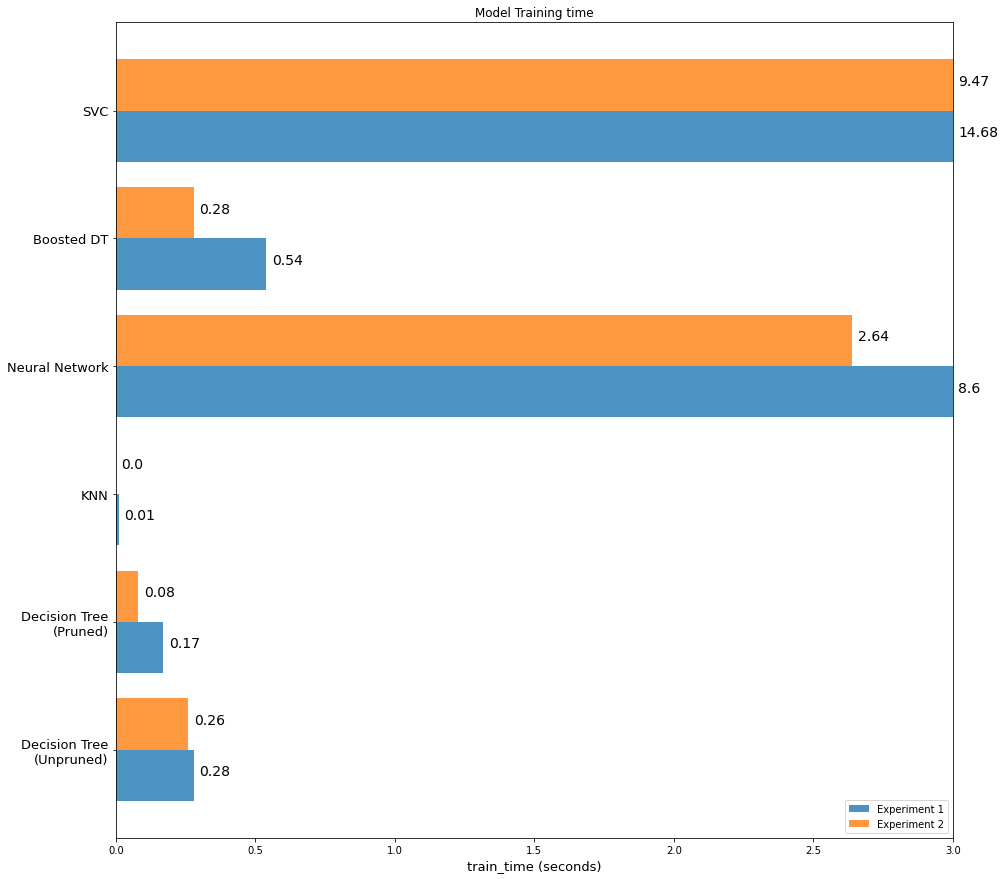
\includegraphics[width=.8\linewidth]{./images/allModelsTrainingTime.png}
			\caption{All supervised learning algorithms timings for training each model. (Full training set)}
			\label{fig:allAgsTrainTime}
		\end{subfigure}
		\begin{subfigure}{.5\textwidth}
			\centering
			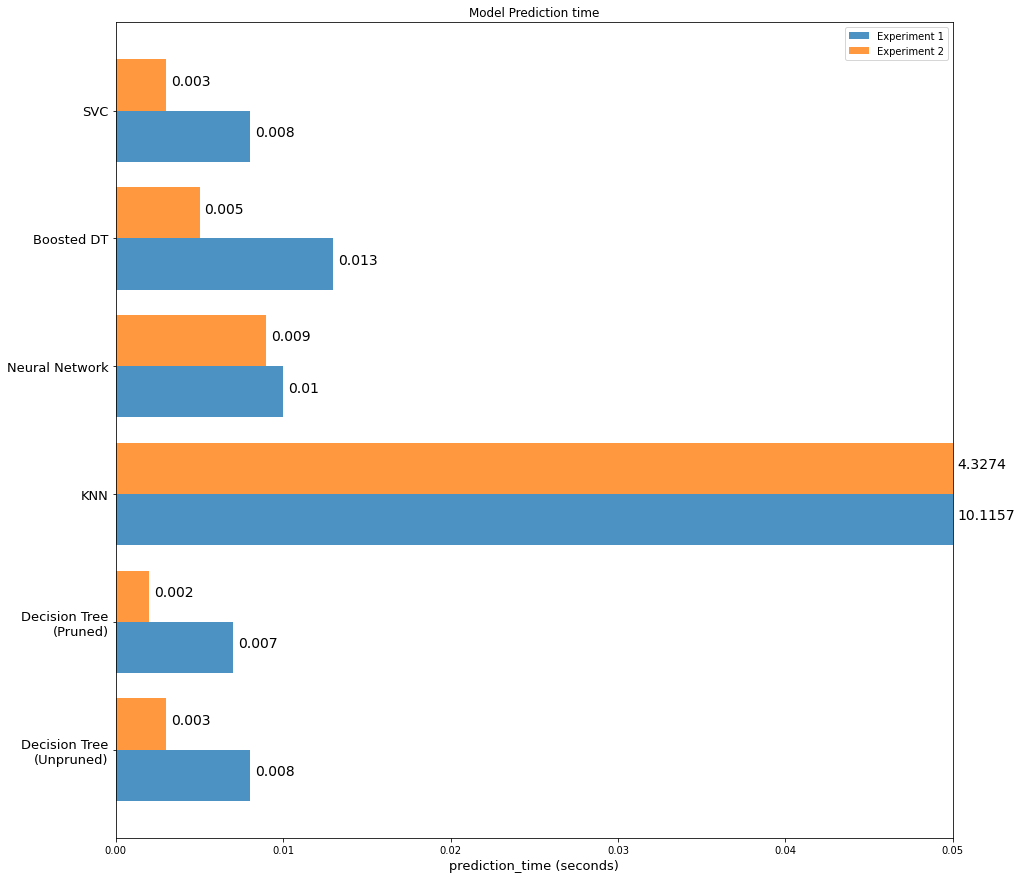
\includegraphics[width=.8\linewidth]{./images/allModelsTestTime.png}
			\caption{Timings for getting predictions on each supervised algorithm. (Full test set)}
			\label{fig:allAgsTestTime}
		\end{subfigure}
	\end{figure}

	\section{Conclusion}
	In this paper we explore multiple supervised learning algorithms, on two data sets in an attempt to see how these algorithms performed on interesting problems. These data sets included multiple possible real life applications including personalized advertisements, and risk management. We used this data to explore five supervised machine learning algorithms consisting of; Decision trees, K-Nearest Neighbors, Neural Networks, Boosted Decision Trees, and Support Vector Classifiers. Each of these algorithms was trained on both data sets and their accuracy was evaluated as amount of training data is increased. Finally after doing this for each algorithm, we looked at all the algorithms compared to each other. Both revisiting the training and testing accuracy, additionally we compared the training, and prediction times for each of the algorithms to gain a deeper understanding of how the algorithms are working under the hood, and what are some trade offs to be made for each of the algorithms.
	
	\nocite{*}
	\printbibliography[
	heading=bibintoc,
	title={References}
	] %Prints the entire bibliography with the title "Whole bibliography"
\end{document}